%%%%%%%%%%%%%%%%%%%%%%%%%%%%%%%%%%%%%%%%%
% Short Sectioned Assignment LaTeX Template Version 1.0 (5/5/12)
% This template has been downloaded from: http://www.LaTeXTemplates.com
% Original author:  Frits Wenneker (http://www.howtotex.com)
% License: CC BY-NC-SA 3.0 (http://creativecommons.org/licenses/by-nc-sa/3.0/)
%%%%%%%%%%%%%%%%%%%%%%%%%%%%%%%%%%%%%%%%%

%----------------------------------------------------------------------------------------
%	PACKAGES AND OTHER DOCUMENT CONFIGURATIONS
%----------------------------------------------------------------------------------------

\documentclass[paper=a4, fontsize=11pt]{scrartcl} % A4 paper and 11pt font size

% ---- Entrada y salida de texto -----

\usepackage[T1]{fontenc} % Use 8-bit encoding that has 256 glyphs
\usepackage[utf8]{inputenc}
%\usepackage{fourier} % Use the Adobe Utopia font for the document - comment this line to return to the LaTeX default

% ---- Idioma --------

\usepackage[spanish, es-tabla]{babel} % Selecciona el español para palabras introducidas automáticamente, p.ej. "septiembre" en la fecha y especifica que se use la palabra Tabla en vez de Cuadro

% ---- Otros paquetes ----

\usepackage{url} % ,href} %para incluir URLs e hipervínculos dentro del texto (aunque hay que instalar href)
\usepackage{amsmath,amsfonts,amsthm} % Math packages
%\usepackage{graphics,graphicx, floatrow} %para incluir imágenes y notas en las imágenes
\usepackage{graphics,graphicx, float} %para incluir imágenes y colocarlas

% Para hacer tablas comlejas
%\usepackage{multirow}
%\usepackage{threeparttable}

%\usepackage{sectsty} % Allows customizing section commands
%\allsectionsfont{\centering \normalfont\scshape} % Make all sections centered, the default font and small caps

\usepackage{fancyhdr} % Custom headers and footers
\pagestyle{fancyplain} % Makes all pages in the document conform to the custom headers and footers
\fancyhead{} % No page header - if you want one, create it in the same way as the footers below
\fancyfoot[L]{} % Empty left footer
\fancyfoot[C]{} % Empty center footer
\fancyfoot[R]{\thepage} % Page numbering for right footer
\renewcommand{\headrulewidth}{0pt} % Remove header underlines
\renewcommand{\footrulewidth}{0pt} % Remove footer underlines
\setlength{\headheight}{13.6pt} % Customize the height of the header

\numberwithin{equation}{section} % Number equations within sections (i.e. 1.1, 1.2, 2.1, 2.2 instead of 1, 2, 3, 4)
\numberwithin{figure}{section} % Number figures within sections (i.e. 1.1, 1.2, 2.1, 2.2 instead of 1, 2, 3, 4)
\numberwithin{table}{section} % Number tables within sections (i.e. 1.1, 1.2, 2.1, 2.2 instead of 1, 2, 3, 4)

\setlength\parindent{0pt} % Removes all indentation from paragraphs - comment this line for an assignment with lots of text

\newcommand{\horrule}[1]{\rule{\linewidth}{#1}} % Create horizontal rule command with 1 argument of height

\graphicspath{ {./images/} }
\usepackage{subcaption}
\usepackage{hyperref}
\usepackage{soul}


%----------------------------------------------------------------------------------------
%	TÍTULO Y DATOS DEL ALUMNO
%----------------------------------------------------------------------------------------

\title{	
\normalfont \normalsize 
\textsc{\textbf{Aprendizaje Automático (2019)} \\ Doble Grado en Ingeniería Informática y Matemáticas \\ Universidad de Granada} \\ [25pt] % Your university, school and/or department name(s)
\horrule{0.5pt} \\[0.4cm] % Thin top horizontal rule
\huge Memoria Práctica 3 \\ % The assignment title
\horrule{2pt} \\[0.5cm] % Thick bottom horizontal rule
}

\author{Luis Balderas Ruiz \\ \texttt{luisbalderas@correo.ugr.es}} 
 % Nombre y apellidos 


\date{\normalsize\today} % Incluye la fecha actual

%----------------------------------------------------------------------------------------
% DOCUMENTO
%----------------------------------------------------------------------------------------

\begin{document}

\maketitle % Muestra el Título

\newpage %inserta un salto de página

\tableofcontents % para generar el índice de contenidos

\listoffigures

\listoftables

\newpage


%----------------------------------------------------------------------------------------
%	Introducción
%----------------------------------------------------------------------------------------

\section{Recognition of handwritten digits}

\subsection{Introducción}

Nos enfrentamos a un problema de clasificación multietiqueta (9 clases, con los números del 0 al 9) (aprendizaje supervisado) sobre una base de datos de reconocimiento de dígitos manuscritos, proveniente de la Universidad de Bogazici. Tras extraer mapas de bits de dimensión $32\times32$ normalizados, se dividen en bloques de $4\times4$ disjuntos y se cuenta el número de píxeles en cada bloque. Esto genera una matriz $8\times8$ con entrada en los números enteros del 0 al 16. Más información en \cite{optdigits.names}. 

\subsection{Preprocesado}

El preprocesado de los datos es la parte más importante del pipeline en un proyecto de ciencia de datos. De él se espera refinar, ajustar, completar y, en definitiva, mejorar la congruencia y consistencia de los mismos para conseguir mejores resultados en la parte de análisis y clasificación. Para conseguir un preprocesado más acertado, me baso continuamente en distintas visualizaciones que arrojen pistas sobre los pasos a seguir. Propongo los siguientes apartados:

\subsubsection{Balanceo de las clases} 

Un dataset balanceado es primordial para garantizar un correcto aprendizaje del modelo. En caso de desbalanceo, las clases más representadas tendrían un peso mayor a la hora de etiquetar instancias nuevas en test, de forma que las menos representadas acabarían, con gran probabilidad, mal clasificadas. Cuando se da desbalanceo hay dos posibles alternativas: eliminar instancias de las clases más repetidas (undersampling) o generar nuevas de las clases minoritarias (oversampling). En este último caso, se suelen utilizar algoritmos como SMOTE (\cite{smote}). \\

En nuestro caso, las clases están absolutamente balanceadas:

\begin{table}[H]
	\centering
	\begin{tabular}{|c|c|}
		\hline
		Etiqueta & Número de instancias \\ \hline
		0        & 178                  \\ \hline
		1        & 182                  \\ \hline
		2        & 177                  \\ \hline
		3        & 183                  \\ \hline
		4        & 181                  \\ \hline
		5        & 182                  \\ \hline
		6        & 181                  \\ \hline
		7        & 179                  \\ \hline
		8        & 174                  \\ \hline
		9        & 180                  \\ \hline
	\end{tabular}
	\caption{Número de instancias por cada clase}
\end{table}

Veámoslo también gráficamente:

\begin{figure}[H] %con el [H] le obligamos a situar aquí la figura
	\centering
	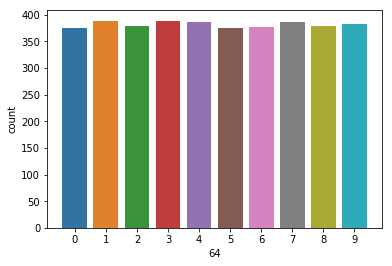
\includegraphics[scale=0.6]{count-clases.png}  %el parámetro scale permite agrandar o achicar la imagen. En el nombre de archivo puede especificar directorios
	\caption{Histograma con el número de instancias por clase} 
	\label{fig:clases}
\end{figure}

Por tanto, no es necesario hacer ninguna modificación en ese sentido.

\subsubsection{Variabilidad de los datos}

A continuación, estudiamos la calidad de las características (columnas en la matriz). Para ello, realizo una descripción estadística de los datos. De las 63 características se estudia la variabilidad de cada individuo a través de la media, la desviación típica, el recorrido intercuartílico, máximo, mínimo... Represento la matriz de correlación para estudiar la correlación lineal entre las características:

\begin{figure}[H] %con el [H] le obligamos a situar aquí la figura
	\centering
	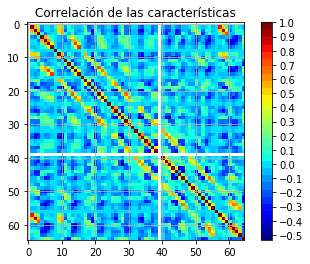
\includegraphics[scale=0.8]{corr-matrix.png}  %el parámetro scale permite agrandar o achicar la imagen. En el nombre de archivo puede especificar directorios
	\caption{Matriz de correlación de características} 
	\label{fig:corr-mat}
\end{figure}

No se aprecia gran correlación lineal entre las variables. Sin embargo, parece que entre la columna 57 y la 1 y la 58 y la 2 (0.822374 y 0.921179 respectivamente) sí hay dependencia lineal.

\subsubsection{Valores perdidos}

Según la documentación del dataset y posteriores análisis exploratorios, no existen valores perdidos en este problema.

\subsubsection{Outliers}

A través de la función definida en el código, basada en el cálculo de $z_{score}$ (\cite{z-score})  para cada instancia, no se ha encontrado ningún outlier. 

\subsubsection{Normalización}

Como se verá en el siguiente apartado, me dispongo a utilizar Análisis de Componentes Principales (PCA) para reducir el tamaño del dataset y optimizar la información. Paso previo a PCA (y también favorable a la clasificación), realizo una normalización y escalado de los datos (\cite{st-sc}). Para ello, lo que se hace es estandarizar las características con una transformación de localización y escala (quitando la media y dividiendo por la desviación típica):

$$ z = \frac{(x-\mu)}{\sigma} $$ 


En clasificadores basados en distancia, es muy importante normalizar los datos, consiguiendo que estén todas en el mismo rango. Ejemplos de ello son k-NN, SVM con núcleo RBF o el propio modelo lineal.

\subsubsection{Selección de instancias}

Dado que el tamaño del dataset no es muy grande, no veo conveniente reducir el número de individuos, por lo que no hago ninguna selección de instancias y trabajaré de forma permanente con todas las filas del conjunto de datos.

\subsubsection{Selección de características: PCA}

Análisis de componentes principales (PCA, \cite{pca}) es una técnica de estadística multivariante basada en describir un conjunto de datos en términos de otras variables nuevas no correladas. Los componentes se ordenan por la cantidad de varianza original que describen, por lo que es una técnica útil para reducir la dimensionalidad de un conjunto de datos. Como ya he comentado antes, PCA requiere una normalización previa de los datos. El motivo es que el algoritmo calcula una nueva proyección del dataset, en la que los ejes están basados en la desviación típica de las variables. Por tanto, si una variable tiene una gran desviación típica, le será asignada un gran peso en el cálculo de ejes, en detrimento de aquellas características que tengan menor variabilidad. En consecuencia, para un análisis verosímil de los datos es necesario que todas las variables tengan la misma desviación típica. Por otra parte, es evidente que cada variable tiene una unidad de medida y hay que garantizar que en el estudio estadístico todas las características se homogeneizan. 

En nuestro problema, aplico PCA con los parámetros 0.95 y svd\_solver == 'full' (\cite{pca-sk}) para que elija el número mínimo de componentes principales de forma que se garantiza una varianza explicada mayor al 95\%. Tras la ejecución, el número de componentes principales encontrada es 41.

\subsection{Sobre métricas para valorar la clasificación(\cite{seleccion-metricas})}

En un problema de aprendizaje supervisado tenemos múltiples formas de evaluar el rendimiento de nuestros modelos. En el fondo, tratamos de ver qué instancias hemos clasificado bien o mal en función de su etiqueta real. Cuando se tienen problemas de clasificación binaria (clase positiva y clase negativa), surgen los siguientes conceptos a la hora de valorar el rendimiento:

\begin{itemize}
	\item Verdaderos positivos (TP): Instancias correctamente clasificadas como positivas.
	\item Verdaderos negativos (TN): Instancias correctamente clasificadas como negativas.
	\item Falsos positivos (FP): Instancias clasificadas como positivas pero que son negativas.
	\item Falsos negativos (FN): Instancias clasificadas como negativas pero que son positivas.
\end{itemize}

La forma de medir el rendimiento más conocida es el llamado Accuracy, que responde a la siguiente fórmula:

$$\text{Accuracy} = \frac{TP+TN}{TP+FP+FN+TN}$$

Sin embargo, dependiendo de la casuística del problema (sobre todo, si las clases están muy desbalanceadas), es posible que esta medida no nos aporte información veraz. Este hecho genera la necesidad de valorar nuevas métricas:

$$\text{Precision} = \frac{TP}{TP+FP}$$

$$\text{Recall} = \frac{TP}{TP+FN}$$

$$\text{F1-score} = \frac{2*\text{Recall}*\text{Precision}}{\text{Recall}+\text{Precision}}$$

Todas ellas generan una visión más precisa de cómo ha sido nuestra clasificación. Por tanto, serán todas añadidas en la sección siguiente tras la ejecución de cada algoritmo. De igual manera, se expresará la matriz de confusión (\cite{cf}).

\subsection{Clasificación}

Esta práctica está centrada en la utilización de modelos lineales. Por tanto, el primer clasificador que voy a utilizar es SGDClassifier de SKLearn (\cite{SGD-C}), esto  es, un modelo lineal basado en gradiente descendente estocástico. Para garantizar una generalización correcta por parte del modelo, utilizo validación cruzada estratificada con 10 particiones(\cite{stk}). Los resultados de los 10 entrenamientos con las distintas particiones son los siguientes: \\

[(1):0.96623376623376622, (2):0.96103896103896103, (3):0.94791666666666663, (4):0.96354166666666663, (5):0.9453125, (6):0.953125, (7):0.93455497382198949, (8):0.9683377308707124, (9):0.9683377308707124, (10):0.95490716180371349] \\


con los siguientes resultados estadísticos:

\begin{itemize}
	\item Media: 0.95633061579731893
	\item Varianza: 0.00012658399732657117
	\item Mínimo: 0.93455497382198949
	\item Máximo: 0.9683377308707124
\end{itemize}

Por tanto, se puede comprobar que se está generalizando bien por la varianza tan pequeña generada y los resultados adquieren mayor credibilidad. Queda tan solo evaluarla en el conjunto de test: \\

\textbf{Accuracy fuera de la muestra:} 0.927657206455.

A continuación, muestro la matriz de confusión:

\begin{figure}[H] %con el [H] le obligamos a situar aquí la figura
	\centering
	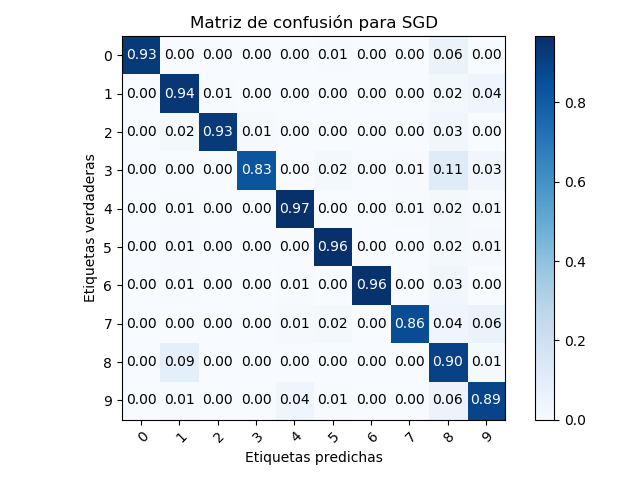
\includegraphics[scale=0.8]{conf-m-sgd.png}  %el parámetro scale permite agrandar o achicar la imagen. En el nombre de archivo puede especificar directorios
	\caption{Matriz de confusión para SGD} 
	\label{fig:conf-m-sgd}
\end{figure}

Para acompañar estas medidas, muestro el resumen completo:

\begin{table}[H]
	\centering
	\begin{tabular}{|c|c|c|c|c|}
		\hline
		& Precision & Recall & F1-Score & Support \\ \hline
		0         & 0.99      & 0.98   & 0.99     & 178     \\ \hline
		1         & 0.86      & 0.91   & 0.88     & 182     \\ \hline
		2         & 0.99      & 0.93   & 0.96     & 177     \\ \hline
		3         & 0.98      & 0.89   & 0.93     & 183     \\ \hline
		4         & 0.93      & 0.96   & 0.95     & 181     \\ \hline
		5         & 0.92      & 0.98   & 0.95     & 182     \\ \hline
		6         & 0.99      & 0.98   & 0.99     & 181     \\ \hline
		7         & 0.98      & 0.88   & 0.93     & 179     \\ \hline
		8         & 0.81      & 0.89   & 0.85     & 174     \\ \hline
		9         & 0.85      & 0.88   & 0.86     & 180     \\ \hline
		avg/total & 0.93      & 0.93   & 0.93     & 1797    \\ \hline
	\end{tabular}
	\caption{Resultados finales de la clasificación con modelo lineal SGD}
\end{table}



A continuación, expreso los resultados del modelo Regresión Logística (\cite{lr}). Realizo de nuevo una validación cruzada con 10 particiones, de forma que obtengo los siguientes resultados: \\

\textbf{Accuracy fuera de la muestra:} 0.943238731219 \\

Matriz de confusión:

\begin{figure}[H] %con el [H] le obligamos a situar aquí la figura
	\centering
	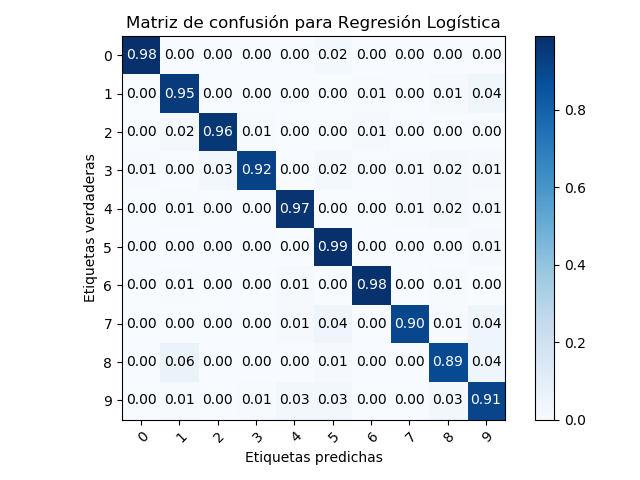
\includegraphics[scale=0.8]{conf-m-rl.png}  %el parámetro scale permite agrandar o achicar la imagen. En el nombre de archivo puede especificar directorios
	\caption{Matriz de confusión para RL} 
	\label{fig:conf-m-rl}
\end{figure}

Finalmente, muestro un resumen de la clasificación por cada una de las clases:

\begin{table}[H]
	\centering
	\begin{tabular}{|c|c|c|c|c|}
		\hline
		& Precision & Recall & F1-Score & Support \\ \hline
		0         & 0.99      & 0.98   & 0.99     & 178     \\ \hline
		1         & 0.91      & 0.95   & 0.92     & 182     \\ \hline
		2         & 0.97      & 0.96   & 0.97     & 177     \\ \hline
		3         & 0.99      & 0.92   & 0.95     & 183     \\ \hline
		4         & 0.95      & 0.97   & 0.96     & 181     \\ \hline
		5         & 0.90      & 0.99   & 0.94     & 182     \\ \hline
		6         & 0.98      & 0.98   & 0.98     & 181     \\ \hline
		7         & 0.99      & 0.90   & 0.94     & 179     \\ \hline
		8         & 0.91      & 0.89   & 0.90     & 174     \\ \hline
		9         & 0.86      & 0.91   & 0.88     & 180     \\ \hline
		avg/total & 0.95      & 0.94   & 0.94     & 1797    \\ \hline
	\end{tabular}
	\caption{Resultados finales de la clasificación con modelo lineal Regresión Lineal}
\end{table}

\newpage

Por último, evalúo el algoritmo SVM (\cite{svc}). Lo primero que hay que hacer es elegir los parámetros con los que se ejecutará el algoritmo. Es necesario elegir $C$ (parámetro de penalización para el término del error), $kernel$ y $gamma$ (coeficiente para el núcleo). Para elegir el mejor conjunto de coeficientes, llevo a cabo un GridSearch con validación cruzada de 10 particiones, asegurando así que elijo los mejores parámetros independientemente de la partición que se haga en los datos. Los mejores resultados son los siguientes:

$$ C = 0.01$$
$$ \gamma = 1^{-9} $$
$$ kernel = linear $$

Con dichos parámetros, se obtienen los siguientes resultados: \\

\textbf{Accuracy fuera de la muestra:} 0.956594323873 \\

Matriz de confusión:

\begin{figure}[H] %con el [H] le obligamos a situar aquí la figura
	\centering
	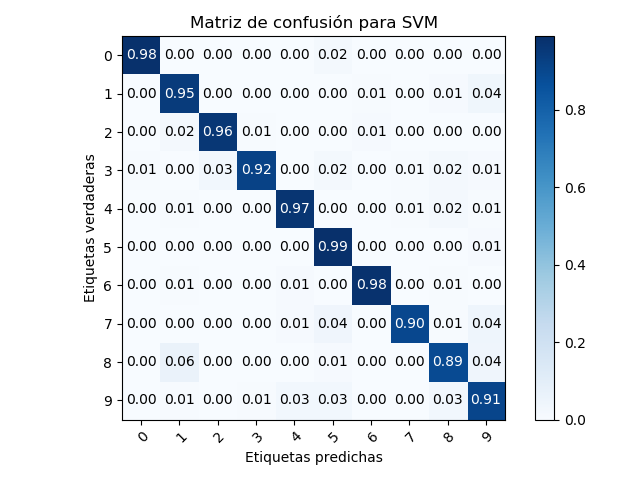
\includegraphics[scale=0.8]{conf-m-svm.png}  %el parámetro scale permite agrandar o achicar la imagen. En el nombre de archivo puede especificar directorios
	\caption{Matriz de confusión para SVM} 
	\label{fig:conf-m-svm}
\end{figure}

\newpage
Resumen de la clasificación:


\begin{table}[H]
	\centering
	\begin{tabular}{|c|c|c|c|c|}
		\hline
		& Precision & Recall & F1-Score & Support \\ \hline
		0         & 0.99      & 0.99   & 0.99     & 178     \\ \hline
		1         & 0.90      & 0.97   & 0.94     & 182     \\ \hline
		2         & 0.96      & 0.97   & 0.96     & 177     \\ \hline
		3         & 0.99      & 0.93   & 0.96     & 183     \\ \hline
		4         & 0.97      & 0.98   & 0.98     & 181     \\ \hline
		5         & 0.95      & 0.98   & 0.97     & 182     \\ \hline
		6         & 1.00      & 0.98   & 0.99     & 181     \\ \hline
		7         & 0.99      & 0.91   & 0.95     & 179     \\ \hline
		8         & 0.96      & 0.89   & 0.92     & 174     \\ \hline
		9         & 0.87      & 0.95   & 0.91     & 180     \\ \hline
		avg/total & 0.96      & 0.96   & 0.96     & 1797    \\ \hline
	\end{tabular}
	\caption{Resultados finales de la clasificación con SVM}
\end{table}

\newpage 
\section{Airfoil self noise}

\subsection{Introducción}

Nos encontramos ante un problema de regresión (aprendizaje supervisado) proveniente de la NASA y alojado en \cite{airfoil-data}. En él se reflejan los datos de una serie de pruebas acústicas y aerodinámicas sobre secciones de aspas en 2 y 3 dimensiones tras ser evaluadas en un túnel de viento. El conjunto de datos consta de 1503 instancias y 6 atributos, que son los siguientes:

\begin{itemize}
	\item Frecuencia (Hertzs)
	\item Ángulo de ataque (grados)
	\item Longitud de la cuerda (metros)
	\item Velocidad de la corriente (m/s)
	\item Espesor de desplazamiento lateral en la succión (en metros)
	\item Nivel de presión de sonido escalado (decibelios) 
\end{itemize}

siendo esta última la salida. En el presente documento se pretende abordar un procesado y análisis de los datos para encontrar una configuración y un regresor óptimo. Comienzo visualizando la distribución de los datos y la correlación lineal de las variables. Los resultados de dicho análisis nos darán idea sobre qué variables son más o menos trascendentes en el estudio. Además, será necesario aplicar normalización sobre los datos, tratamiento de outliers o valores perdidos.

\newpage

\subsection{Preprocesado}

En primer lugar, muestro la matriz de correlación de las variables junto con el coeficiente correspondiente.
\begin{figure}[H] %con el [H] le obligamos a situar aquí la figura
	\centering
	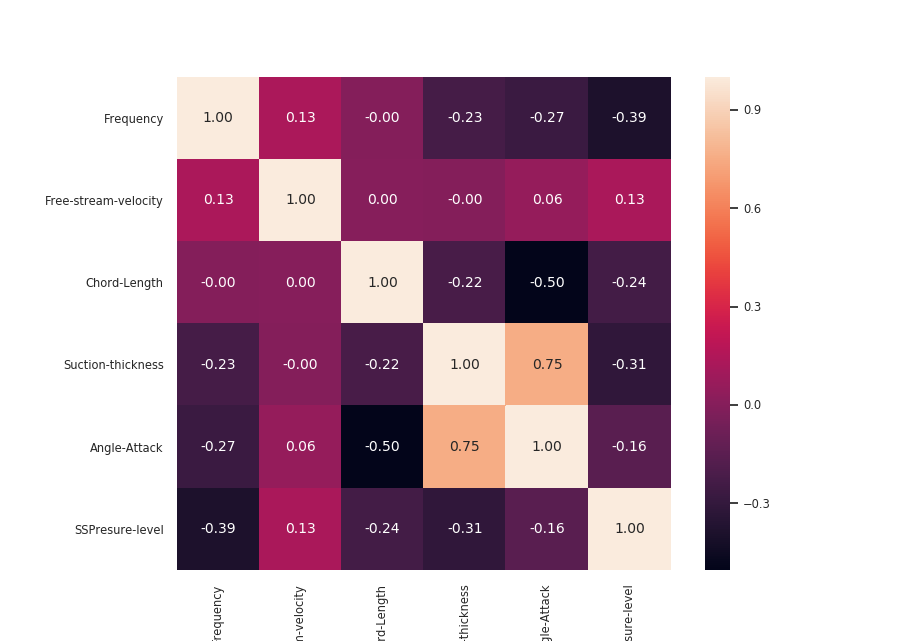
\includegraphics[scale=0.6]{corr-airfoil.png}  %el parámetro scale permite agrandar o achicar la imagen. En el nombre de archivo puede especificar directorios
	\caption{Matriz de correlación entre las variables} 
	\label{fig:corr-airfoil}
\end{figure}

Como se puede comprobar, la correlación lineal entre las variables es baja. Eso nos indica que el dataset no es redundante y que todas las variables nos aportarán información por sí solas. Tan sólo podemos encontrar dos variables que sí tienen una alta correlación entre ellas: 'Suction-thickness' y 'Angle-Attack', con 0.75 de coeficiente de correlación lineal. Por tanto, podríamos plantearnos eliminar alguna de ellas porque son mutuamente explicables. Además, 'Suction-thickness' Y 'Chord-length' mantienen una correlación inversa de 0.5. 

Para obtener más información, visualizo la distribución de las variables y su relación a través de un pairplot.

\begin{figure}[H] %con el [H] le obligamos a situar aquí la figura
	\centering
	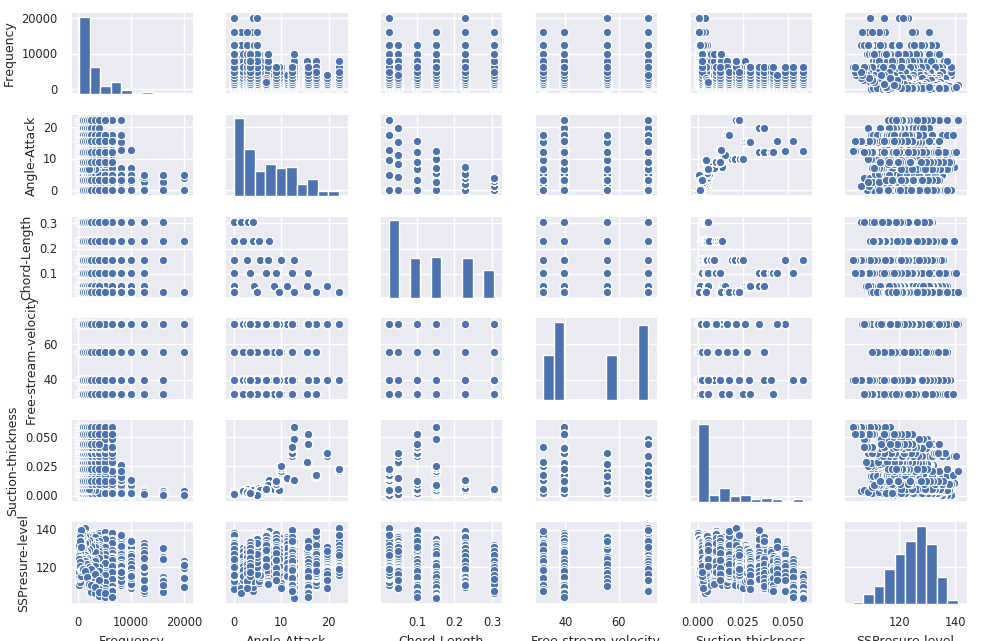
\includegraphics[scale=0.6]{pairplot-air.png}  %el parámetro scale permite agrandar o achicar la imagen. En el nombre de archivo puede especificar directorios
	\caption{Pairplot para el dataset Airfoil} 
	\label{fig:pairplot-air}
\end{figure}

Podemos ver ahora con más claridad la correlación entre las variables antes comentadas. Por tanto, podremos considerar la eliminación de alguna de esas características.

\subsubsection{Outliers}

Seguidamente, muestro un resumen estadístico de las variables:

\begin{table}[H]
	\resizebox{16cm}{!}{
	\begin{tabular}{|c|c|c|c|c|c|c|}
		\hline
		& Frequency & Angle-Attack & Chord-Length & Free-Stream Velocity & Suction-tickness & SSPresure-level \\ \hline
		count & 1.00      & 1503         & 1503         & 1503                 & 1503             & 1503            \\ \hline
		mean  & 0.92      & 2886.380572  & 0.136548     & 50.860745            & 0.01114          & 124.835943      \\ \hline
		std   & 0.99      & 3152.573137  & 0.093541     & 15.572784            & 0.01315          & 6.898657        \\ \hline
		min   & 0.99      & 200          & 0.0254       & 31.7                 & 0.000401         & 103.38          \\ \hline
		25\%  & 0.95      & 800          & 0.0508       & 39.6                 & 0.002535         & 120.191         \\ \hline
		50\%  & 0.93      & 1600         & 0.1016       & 39.6                 & 0.004957         & 125.721         \\ \hline
		75\%  & 1.00      & 4000         & 0.2286       & 71.3                 & 0.015576         & 129.9955        \\ \hline
		max   & 0.98      & 20000        & 22.2         & 71.3                 & 0.058411         & 140.987         \\ \hline
	\end{tabular}}
	\caption{Resumen estadístico de las variables}
\end{table}

Como vemos, la variable 'Frequency' es la que más desviación típica tiene, por lo que podría generar más outliers. Me centro en esa característica y la comparo con nuestro target, para ver si hay datos que se desvían mucho:

\begin{figure}[H] %con el [H] le obligamos a situar aquí la figura
	\centering
	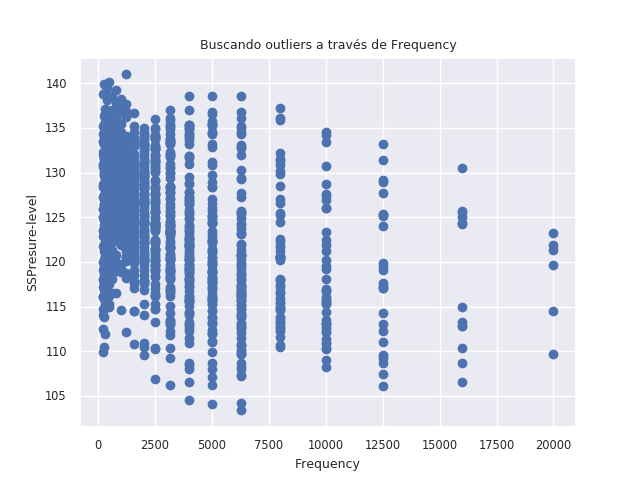
\includegraphics[scale=0.6]{freq-ssp.png}  %el parámetro scale permite agrandar o achicar la imagen. En el nombre de archivo puede especificar directorios
	\caption{Relación entre la variable Frequency y SSPresure-Level} 
	\label{fig:freq-ssp}
\end{figure}



\newpage
\section{Bibliografía}

%------------------------------------------------

\bibliography{citas} %archivo citas.bib que contiene las entradas 
\bibliographystyle{plain} % hay varias formas de citar

\end{document}
